\documentclass[]{beamer}
\usetheme{Singapore}
\usepackage{hyperref}
\usepackage{helvet}
\usepackage{graphicx}
\usepackage{array}
\usepackage{tipa}
\usepackage{booktabs}
\usepackage[small,nohug,heads=vee]{diagrams}
\usepackage[normalem]{ulem}

\mode<presentation>
\title{Using Speech Community Data as Phonological Evidence}
\author{Josef Fruehwald}
\institute{University of Pennsylvania}
\date{September 16, 2011\\Penn State, The Center for Language Science}



\AtBeginSection[]
{
  \begin{frame}<beamer>{Outline}
    \tableofcontents[currentsection]
  \end{frame}
}



\usepackage{Sweave}
\begin{document}
\begin{frame}
	\titlepage
\end{frame}

\section{Introduction}

\subsection{Motivations}

\begin{frame}
	\frametitle{Motivations}
	\framesubtitle{Phonological Context}
	
	\begin{block}{``Classic'' Evidence}
		\begin{itemize}
			\item Alternations / Static Distributions.
			\item Drawn from introspection / Small number of informants.
		\end{itemize}
	\end{block}
	
	\begin{block}{LabPhon}
		\begin{itemize}
			\item Experimental Measures (acoustic, articulatory, judgments).
			\item Drawn from standard pools of experimental subjects.
			\item Frequently expressing concerns about the validity of Classic phonological evidence.
		\end{itemize}
	\end{block}
	
\end{frame}

\begin{frame}
	\frametitle{Motivations}
	\framesubtitle{Sociolinguistic Context}
	
	\begin{block}{Linguistic Theory}
		\begin{itemize}
			\item Variable Rules
			\item Lexical Phonology (Guy, 1991a;b)
			\item Exemplar Theory
		\end{itemize}
	\end{block}
	
	\begin{block}{Variation Theory}
		\begin{itemize}
			\item What is changing where, and how?
			\item What can influence variation?
		\end{itemize}
	\end{block}
	
	\begin{block}{Social Theory}
		\begin{itemize}
			\item How does one construct and project their identity?
		\end{itemize}
	\end{block}
\end{frame}

\begin{frame}
	\frametitle{Motivations}
	\framesubtitle{Sociolinguistic Context}
	\begin{block}{Research Focus of Papers in the Proceedings of NWAV}
		\begin{center}
		\begin{tabular}{rrrrr}
			\toprule
						&Linguistic & Variation & Social & Etc.\\
			\cmidrule{2-5}
			NWAV 37 &      2         &   8       &   4       & --      \\
			NWAV 38 &     1          &     12 &    4     &   2   \\
			\bottomrule
		\end{tabular}
		\end{center}
	\end{block}
\end{frame}

\begin{frame}
	\frametitle{Motivations}
	\framesubtitle{Using Variation for Phonological Argument}
	
	\begin{block}{Andries Coetzee}
		\begin{itemize}
			\item [$\sim$] Frequency biases in phonological variation, {\it NLLT} (w/ Shigeto Kawahara)
			\item [$\sim$] The place of variation in phonological theory, {\it The Handbook of Phonological Theory. 2nd Edition} (w/ Joe Pater)
			\item [$\sim$] \ldots
		\end{itemize}	
	\end{block}
	
	\begin{block}{Ricardo Berm\'udez-Otero}
		\begin{itemize}
			\item [$\sim$] Cycles and continua: on unidirectionality and gradualness in language change {\it Handbook on the history of English} (w/ Graeme Trousdale)
			\item [2007] Diachronic phonology {\it The Cambridge handbook of phonology}
			\item [$\sim$] \ldots
		\end{itemize}
	\end{block}
\end{frame}


\subsection{Goals}

\begin{frame}
	\frametitle{Goals}
	
	\begin{itemize}
		\item Identify how sociolinguistic data can be used for phonological theory building.
		\item Identify how sociolinguistic data can be used for identifying and specifying phonological phenomena.
		\item Identify the ways in which sociolinguistic data achieves these goals uniquely.
	\end{itemize}

\end{frame}

\subsection{Data}

\begin{frame}{Data Sources}

	\begin{block}{Philadelphia Corpus}
		Automatically extracted vowel measurements from 272 Philadelphia speakers interviewed between 1973 and 2010. Dates of birth
		ranging from 1888 to 1991.
	\end{block}
	
	\begin{block}{Atlas of North American English}
		Acoustic vowel measurements from survey respondents in the Atlas of North American English.
	\end{block}

	\begin{block}{Sociolinguistic Literature}
		Various accounts of sound change in progress from the sociolinguistic literature.
	\end{block}



\end{frame}

\begin{frame}{Philadelphia Corpus}
	\framesubtitle{FAAV Project}
%	\begin{columns}[c]
	
%	\column{1.5in}
	\begin{diagram}
		\raisebox{-.5\height}{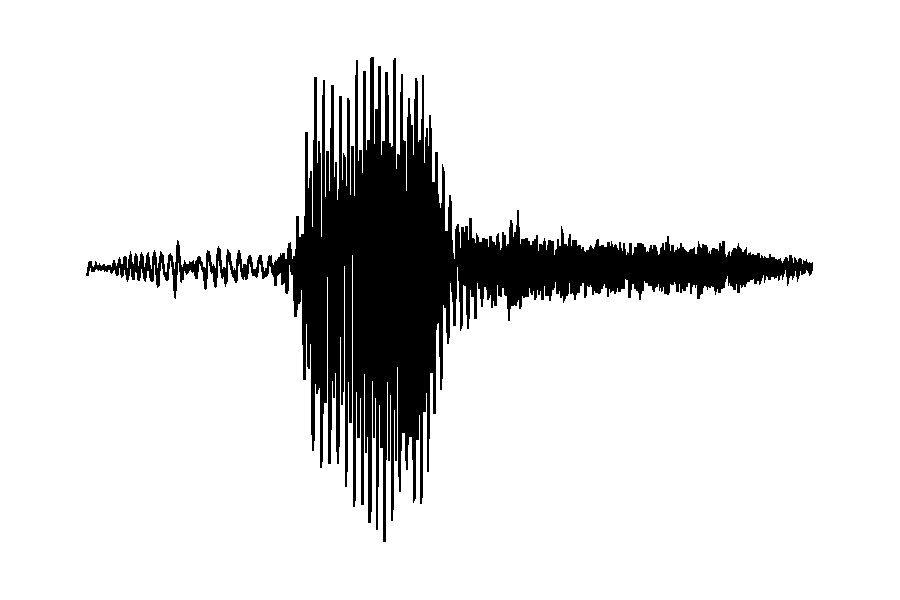
\includegraphics[width = 0.1\textwidth]{figures/wav.pdf}} &&
		\raisebox{-.5\height}{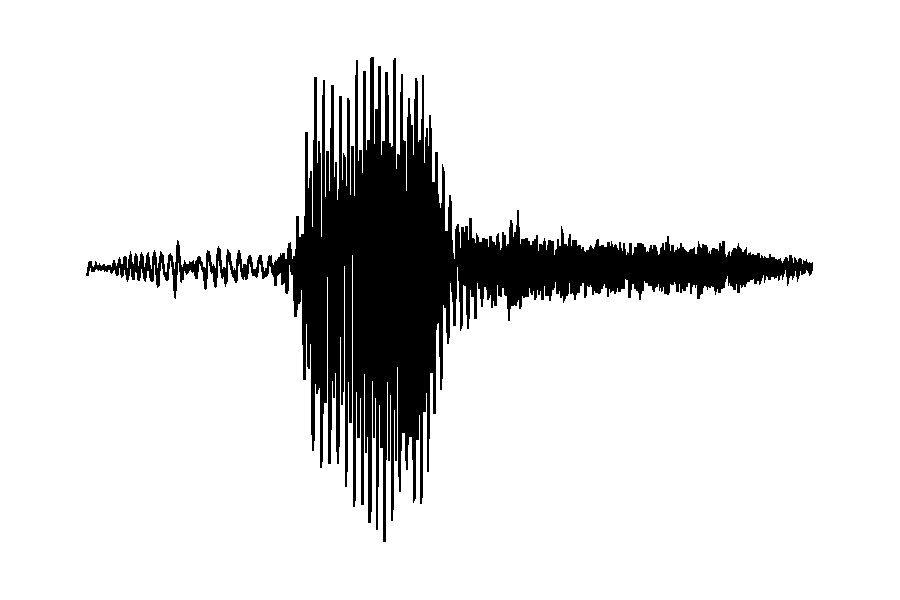
\includegraphics[width = 0.1\textwidth]{figures/wav.pdf}} + \fbox{transcription} &&
		\raisebox{-.5\height}{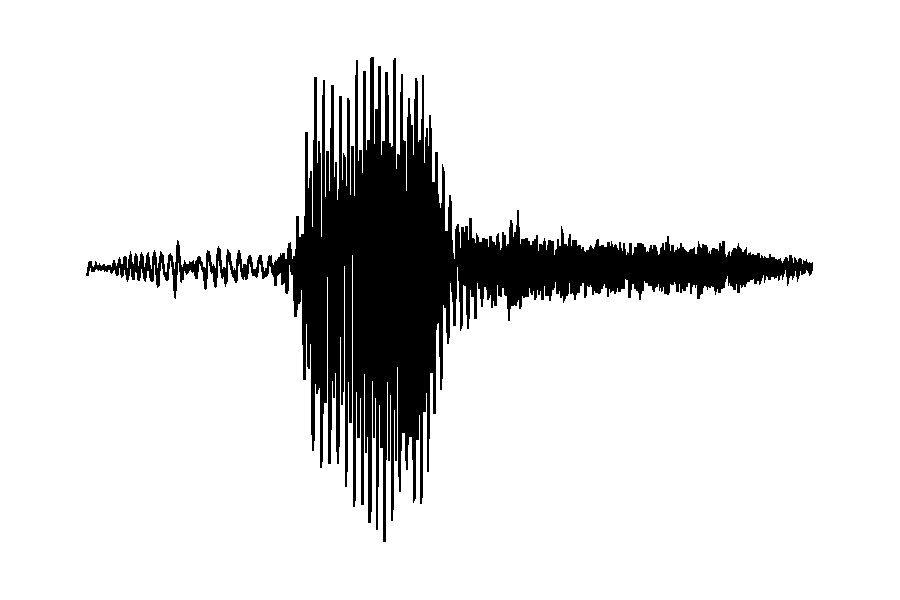
\includegraphics[width = 0.1\textwidth]{figures/wav.pdf}} + \fbox{forced\vphantom{g}}\fbox{alignment}\\
		 \dTo &\ruTo(2,3) & \dTo_{P2FA} & \ruTo(2,3) & \dTo_{extractFormants}\\
		 		&&	&&\\
		\fbox{transcription} &\phantom{what}& \fbox{forced\vphantom{g}}\fbox{alignment} &\phantom{what}&\raisebox{-.5\height}{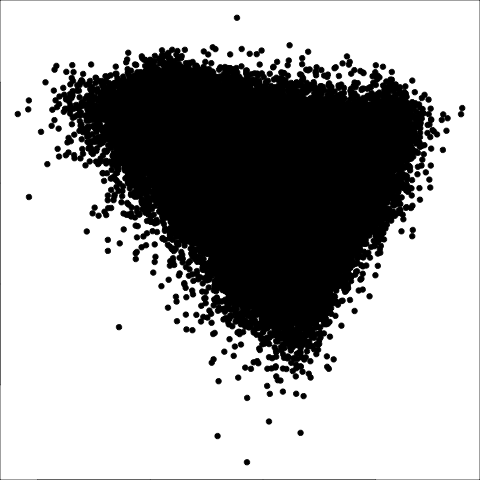
\includegraphics[width = 0.2\textwidth]{figures/vowels.png}} \\
	\end{diagram}
	

\end{frame}

%% Motivation:
%%	Classical / Laboratory Phonology
%%	Naturalistic language observation is also useful / crucial\

%% Outline:
%%	Establish a linking hypothesis between observable phonetic variation and phonological structure
%%		Universal Phonetics vs. Langauge Specific Phonetics vs. Exemplar Theory
%%	Case Study

\section{Phonology-Phonetics Interface}

\begin{frame}{Phonology-Phonetic Interface}

	\begin{block}{Options}
		\begin{itemize}
			\item Universal Phonetic Implementation
			\item Langauge Specific Phonetic Implementation
			\item Exemplar Theory
		\end{itemize}
	\end{block}

\end{frame}

\begin{frame}{Phonology-Phonetic Interface}
	
	\begin{block}{Linking Hypothesis}
		All I have to work with is phonetic measurements, so settling on a PH-interface model
		is crucial in order to make any connection to phonological theory at all.
	\end{block}

\end{frame}

\subsection{Universal Phonetic Implementation}



\setkeys{Gin}{with = 0.8\textwidth}

\begin{frame}{Phonology-Phonetic Interface}
	\framesubtitle{Continuous Change}

\includegraphics{fruehwald_CLS_2011-002}
	
	
\end{frame}



\begin{frame}{Phonology-Phonetic Interface}
	\framesubtitle{Continuous Change}

\includegraphics{fruehwald_CLS_2011-004}
	
	
\end{frame}

\begin{frame}{Phonology-Phonetic Interface}

	\begin{block}{Options}
		\begin{itemize}
			\item \sout{Universal Phonetic Implementation}
			\item Langauge Specific Phonetic Implementation
			\item Exemplar Theory
		\end{itemize}
	\end{block}

\end{frame}

\subsection{Exemplar Theory}

\begin{frame}{Phonology-Phonetics Interface}
	\framesubtitle{Category Shifts}
	

\end{frame}


\subsection{Language Specific Phonetics}





\section{Identifying Phonological Processes}



\subsection{/ey/ Introduction}

\subsection{Analysis}


\begin{frame}{Phonology-Phonetic Interface}
	\framesubtitle{Syllabic Context}

\includegraphics{fruehwald_CLS_2011-007}
	
\end{frame}


\begin{frame}{Phonology-Phonetic Interface}
	\framesubtitle{Segmental Context}

\includegraphics{fruehwald_CLS_2011-009}
		
\end{frame}




\begin{frame}{Phonology-Phonetic Interface}
	\framesubtitle{Morphological Interaction}

\includegraphics{fruehwald_CLS_2011-012}
		
\end{frame}




\begin{frame}{Phonology-Phonetic Interface}
	\framesubtitle{Morphological Interaction}

\includegraphics{fruehwald_CLS_2011-014}
		
\end{frame}



\subsection{Phonological Description}


\subsection{The Unique View of Diachrony}

\section{Conclusion}





\end{document}  
